\chapter{Preparatory Work}\label{ch:samples}
This chapter describes the preparatory work done on the the data and Monte Carlo samples used for the cross section analyses. This entails:

\begin{enumerate}
\item the MC production,
\item the energy calibration of the detector both in data and MC,
\item the optimization of the tracking algorithm for the total cross section analyses.
\end{enumerate}

\section{Construction of a Monte Carlo Simulation for LArIAT}
\subsection{G4Beamline}\label{ch:beamlineComposition}
\subsection{Data Driven MC}\label{sec:DDMC}

\section{Tracking Studies}

\section{Energy Calibration and Studies}

\section{Estimate of Energy Loss before the TPC}

\begin{comment}
\section{Construction of a Monte Carlo Simulation for LArIAT}
For the simulation of LArIAT events and their particle make up, we use a combination of two MC generators: the G4Beamline Monte Carlo and the Data Driven single particle Monte Carlo (DDMC). We use the G4Beamline MC to simulate the particle transportation in the beamline and calculate the particle composition of the beam just past the fourth Wire Chamber (WC4). In order to simulate the beam line particles after WC4 and in the TPC, we use the DDMC.
\subsection{G4Beamline}\label{beamlineComposition}
G4Beamline simulates the beam collision with the LArIAT secondary target, the energy deposited by the particles in the LArIAT beamline detectors and the action of the LArIAT magnets, effectively accounting for particle transportation through the beam line from the LArIAT target until ``Big Disk", a fictional, void detector located just before the cryostat. 
 At the moment of this writing, G4Beamline does not simulated the responses of the beam line detectors. It is possible to interrogate the truth level information of the simulated particles in several points of the geometry. In order to ease the handshake between G4Beamline and the DDMC, we ask for the beam composition just after WC4.
Since LArIAT data are taken under different beam conditions, G4Beamline simulates separately the beam composition according to the magnets' settings and the secondary beam intensity. For the pion cross section analysis the relevant beam conditions are  secondary beam energy of 64 GeV, negative polarity magnet with current of 100 A and 60 A. For the kaon cross section analysis the relevant beam conditions is a secondary beam energy of 64 GeV, positive polarity magnet with current of 100 A. 

\textcolor{red}{DECIDE IF YOU WANT THE BEAM COMPOSITION HERE}
%Figure 16 shows the tertiary beam spectra for the 64 GeV and 100 A. 

%In Table 3, the beam composition is given in terms of percentage of different particle species per spill for positive polarity. The values reported are the weighted average on the two beam conditions considered. The weights are calculated according to the fourth column of Table 2.

\subsection{Data Driven MC}\label{sec:DDMC}
The Data Driven single particle Monte Carlo (DDMC) is a single particle MC gun which simulates the particle transportation from WC4 into the TPC leveraging on the beamline data information. The DDMC uses the data momentum and position at WC4 to derive its initial conditions: a general sketch of the DDMC workflow is shown in Figure \ref{fig:DDMCSketch}.

When producing a DDMC sample, beam line data from a particular running period and/or running condition are selected first. Figure \ref{fig:DDMCQuantities}  schematically shows the data quantities of interest leveraged from data: the momentum ($P_x, P_y, P_z$) and position ($X, Y$) at WC4. For each data event, we obtain the particle position ($X, Y$) at WC4 directly from the data measurement. On the contrary, we calculate the components of the momentum using the beamline measurement of the momentum magnitude (see section \ref{sec:MWPCfunc}) in conjunction with the hits on WC3 and WC4 to determine the direction of the momentum vector, as described in \ref{sec:MWPCfunc}. The momentum and position of the selected data is sampled thousand of times through a 5-dimensional hit-or-miss sampling procedure. This produces MC distributions with the same momentum and position distributions as data, with the additional benefit of accounting for the correlations between the considered variables. A LArSoft simulation module then launches single particle MC from z = -100 cm (the location of the WC4) using the sampled momentum and position distributions as a template. 
As an example, the results of the DDMC generation compared to data for the pion 60A sample are shown in figure \ref{DDMCComparison}; as expected, MC and data agree within the statistical uncertainty by construction. Using this technique ensures the MC and data particles have very similar momentum, position and angular distributions at WC4 and allow us to us the MC sample in several occasions, for example to calibrate the energy loss upstream of the TPC or account for the WC2TPC match inefficiency. A small caveat is in order here: the DDMC is a single particle Monte Carlo, which means that the beam pile-up is not simulated. 
Three sample of \textcolor{red}{NUMBERS} pions, muons and electrons, as well as  a sample of \textcolor{red}{NUMBERS} kaons have been generated with the DDMC and are used for the MC cross section study.

\begin{figure}[hpbt]
\centering
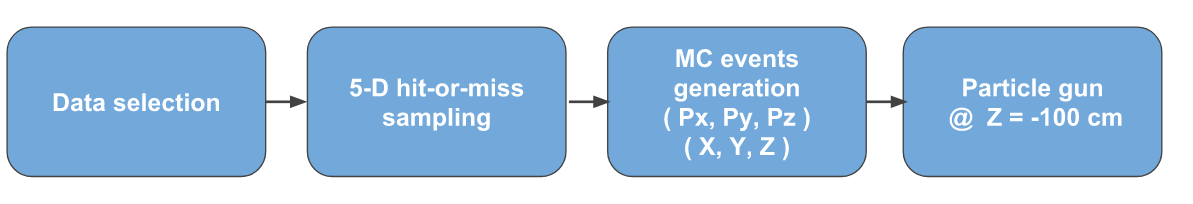
\includegraphics[width=\textwidth]{Chapter-5/Images/DDMCScheme.png}
\caption{Workflow for Data Driven single particle Monte Carlo production.}
\label{fig:DDMCSketch}
\end{figure}


\begin{figure}[hpbt]
\centering
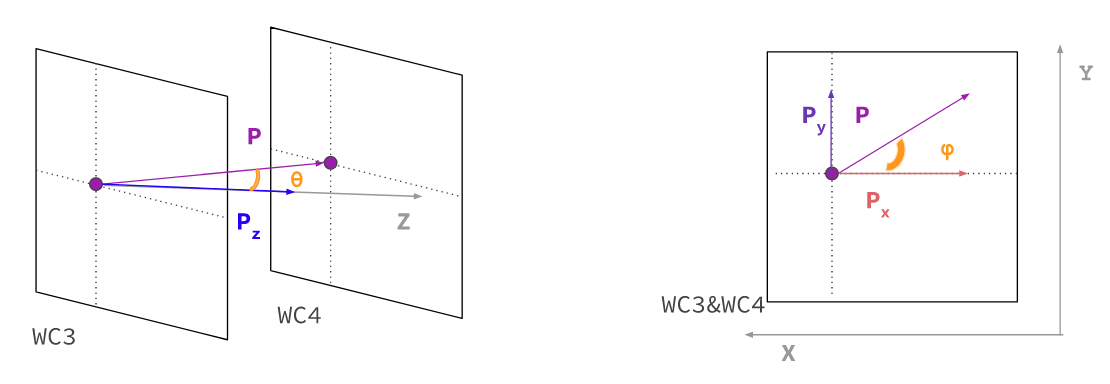
\includegraphics[width=\textwidth]{Chapter-5/Images/DDMCQuantities.png}
\caption{Scheme of the quantities of interest for the DDMC event generation: $P_x, P_y, P_z, X, Y$ at WC4.}
\label{fig:DDMCQuantities}
\end{figure}


\begin{figure}[hpbt]
\centering
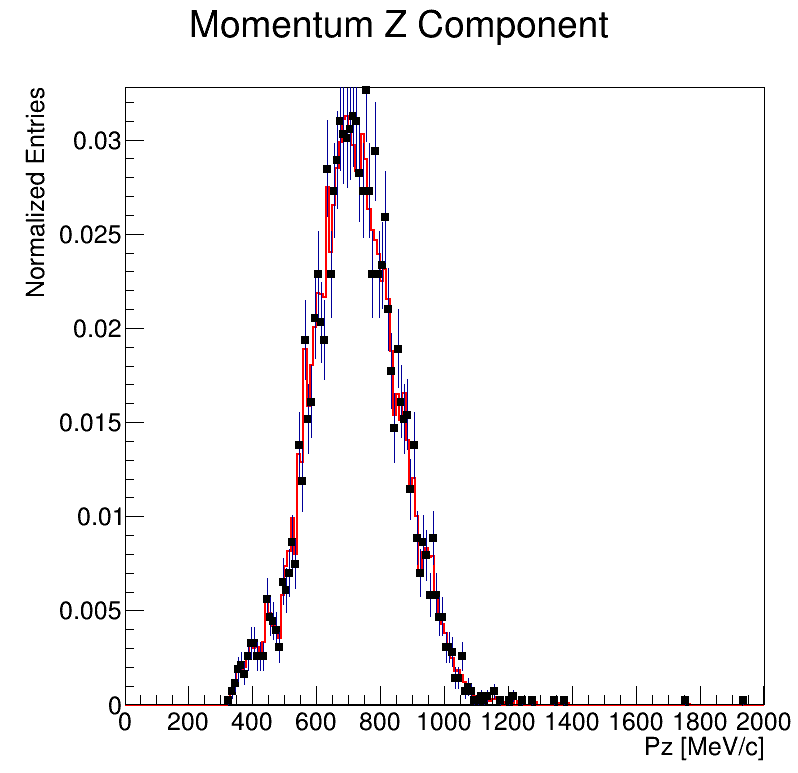
\includegraphics[width=\textwidth]{Chapter-5/Images/Pz.png}
\caption{Comparison between generated quantities and data distributions for the 60A pion sample: Z component of the momentum (top left), X position at Wire Chamber 4 (top right), Y position at Wire Chamber 4 (bottom).}
\label{fig:DDMCComparison}
\end{figure}



%%%%%%%%%%%%%%%%%%%%%%%%%%%%%%%%%%%%%%%%%%%
%%%%%%%%%%%%%%         Energy Calibration         %%%%%%%%%%%%%%         
%%%%%%%%%%%%%%%%%%%%%%%%%%%%%%%%%%%%%%%%%%%
\section{Energy Calibration}\label{ch:energyCalibration}
Scope of the energy calibration is to identify the factors which convert the charge collected (dQ) to energy deposited in the chamber(dE). As described in section \ref{sec:SignalProc}, this is a multi-step procedure. In LArIAT, we first correct the raw charge by the electronic noise on the considered wire \cite{technote}, then by the electron lifetime \cite{LArIATLifeTime},  and then by the recombination using the ArgoNeut recombination values. Lastly, we apply overall calibration of the energy, i.e. we determine the ``calorimetry constants" using the procedure described in this section.


We independently determine  the calorimetry constants for Data and Monte Carlo in the LArIAT Run-II Data samples using  a parametrization of the energy deposited per unit length (dE/dX) as a function of momentum. This is done by comparing the stopping power measured on reconstructed quantities against the Bethe-Bloch theoretical prediction for various particle species (see equation \ref{eq:BB}).  We obtain the theoretical expectation for the dE/dX most probable value of pions ($\pi$), muons ($\mu$), kaons ($K$), and protons ($p$) in the momentum range most relevant for LArIAT (Figure \ref{fig:PDGEnergyLossArgon}) using the tables provided by the Particle Data Group \cite{Patrignani:2016xqp} for liquid argon \cite{PDG-Argon}.

The basic idea of this calibration technique is to utilize the most upstream portion of a TPC track which has a well known momentum and particle species to measure its $dE/dX$. Once a sample of particles dE/dX has been measured at various momenta, we then tune to calorimetry constants within the reconstruction software to align these measured values to match the theoretical ones found in Figure \ref{fig:PDGEnergyLossArgon}. 

In data, we start by selecting a sample of beamline positive pion candidates without any restriction on their measured momentum.
We then apply the WC2TPC match and subtract the energy loss upstream to the TPC front face, determining the momentum at the TPC front face. For each surviving pion candidate,  we measure the dE/dx at each of the first 12 spacepoints associated the 3D reconstructed track, corresponding to a $\sim$ 5 cm portion. These dE/dX measurements are then put into a histogram that corresponds to measured momentum of the track. The dE/dX histograms are sampled every 50 MeV in momentum (e.g. 150~MeV/c $< P <$ 200~MeV/c, 200~MeV/c $< P <$ 250/c~MeV, etc...).   This process of selecting, sampling, and recording the dE/dX for various momentum bins is repeated over the entire sample of events, allowing us to collect sufficient statistic in most of the momentum bins between 150~MeV/c and 1100~MeV/c.
Each 50 MeV/c momentum binned dE/dX histogram is now fit with a simple Landau function. The most probable value (MPV) and the associated error on the MPV from the fit are extracted and plotted on Figure \ref{fig:PDGEnergyLossArgon}. Depending on the outcome of the fit, we modify the calorimetry constants and we repeat the procedure until a qualitative agreement is achieved.  We perform this  tuning for the collection and induction plane separately. 
As a cross check to the determined calorimetry constants using the positive pions, we plot the dE/dx vs momentum distribution all the other particle species identifiable in the beamline data ($\pi$, K , p, in both polarities) against the corresponding Beth-Bloch prediction in a similar fashion. On average, pions and muons only lose $\sim$10 MeV in this 5~cm section of the track and protons lose $\sim$20 MeV. Thus choosing 50 MeV size bins for our histograms covers the energy spread within those bins due to energy loss from ionization.  The results of the tuning and cross check for Run-II data on the collection plane is shown in Figure \ref{fig:BBandData} positive polarity data on the left, negative polarity data on the right.

In MC, we simulate the corresponding positive pion sample with the DDMC (see section \ref{sec:DDMC}) and follow the same steps as in data. The calorimetry tuning is explained in all his gory details in \cite{technote}.


\begin{figure}[htb]
\centering
%\includegraphics[width=0.50\textwidth]{images/PDGdEdX.png}
\caption{Mean energy loss in various materials over a range of particle momenta as produced in Reference \cite{PDG}.}
\label{fig:PDGEnergyLoss}
\end{figure}


\begin{figure}[htb]
\centering
%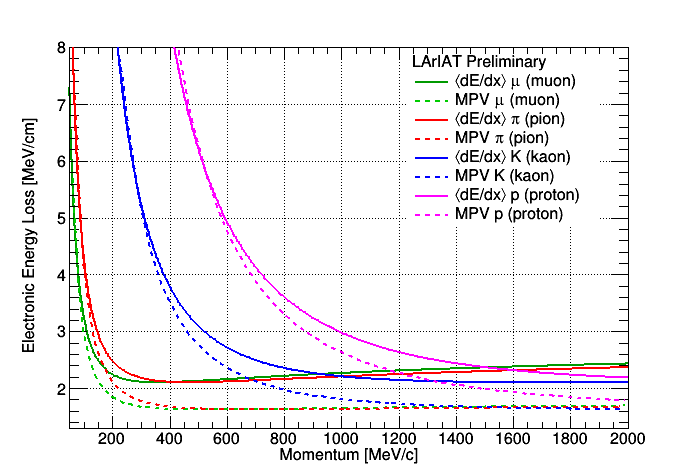
\includegraphics[width=0.50\textwidth]{images/dEdXvsMomentumTemplate}
\caption{Mean energy loss for pions, muons, and protons in liquid argon over the momentum range most relvant for LArIAT.}
\label{fig:PDGEnergyLossArgon}
\end{figure}




\begin{figure}[htb]
\centering
%\includegraphics[width=0.50\textwidth]{images/CalibrationExample.png}
\caption{Illustration of the calibration technique. Here we depict a 325 MeV wire chamber track (shown in green) which enters the TPC (taking into account the energy loss from the upstream material) and we sample the first 12 spacepoints (shown in teal) to extract the dE/dX distribution which is fit with a Landau.}
\label{fig:CalibrationExample}
\end{figure}





%%%%%%%%%%%%%%%%%%%%%%%%%%%%%%%%%%%%%%%%%%%
%%%%%%%%%%%%%%         Energy Calibration         %%%%%%%%%%%%%%         
%%%%%%%%%%%%%%%%%%%%%%%%%%%%%%%%%%%%%%%%%%%




\section{Tracking Studies}
In this section, we describe three studies. The first is a justification of the selection criteria for the beamline handshake with the TPC information.  We perform this study to boost  the correct identification of the particles in the TPC associated with the beamline information, while maintaining sufficient statistics for the cross section measurement. 
The second study is an optimization of the tracking algorithm, with the scope of maximizing the identification of the hadronic interaction point inside the TPC. These two studies are related, since the optimization of the tracking is performed on TPC tracks which have been matched to the wire chamber track; in turn, the tracking algorithm for TPC tracks determine the number of reconstructed tracks in each event used to try the matching with the wire chamber track. Starting with a sensible tracking reconstruction, we perform the WC2TPC matching optimization first, then the tracking optimization. The WC2TPC match purity and efficiency  are then calculated again with the optimized tracking.


%\section{MC sample and WC2TPC match}
We perform the following studies on a MC sample of 191000 kaons and 359000 pions produced with the DDMC technique. DDMC particles are shot from the WC4 location into the TPC following the beam profile.
We mimic the matching between the WC and the TPC track on Monte Carlo by constructing a fake WC track using truth information at wire chamber four. We then apply the same WC to TPC matching algorithm as in data described in \ref{ch:WC2TPCMatchMethod}. 



%In data, we attempt to uniquely match one WC-Track to one and only one reconstructed TPC track. This match is done by using in the $X$ and $Y$ coordinate of the extrapolated WC-Track to the upstream most point of the reconstructed TPC Track and by using the angle between the incoming track angle and the reconstructed TPC. We define $\Delta$X as the difference between the $x$ position of the most upstream point of the TPC track and the $x$ position of the WC track as projected to the TPC front face. $\Delta$Y is defined analogously. We define  $\Delta$R as $ \Delta \text{R} =  \sqrt{ \Delta \text{X}^2 +  \Delta \text{Y}^2}  $. The angle between the incident WC Track and the TPC track in the plane that contains them defines $\alpha$.  

%We define a match between WC-track and TPC reconstructed track if  $\Delta \text{R} < r_{T}$, $\alpha < \alpha_{T}$ and the Z position of the first reconstructed point of the TPC track is within 2 cm from the TPC front face. The determination of the best $r_{T}$ and $\alpha_{T}$ is the scope of the following section.

%In MC, we mimic the matching between the WC and the TPC track on Monte Carlo by constructing a fake WC track using truth information at wire chamber four. We then apply the same WC to TPC matching algorithm as in data. 

\subsection{Selection Study for the Wire Chamber to TPC Match}\label{ch:WC2TPCMatchOptimization}
Plots I want in this section:
\begin{enumerate}
\item WC2TPC MC DeltaX, DeltaY and $\alpha$
\end{enumerate}


Scope of this study is assessing the goodness of the wire chamber to TPC match on Monte Carlo and decide the selection values we will use on data. A word of caution is necessary here. With this study, we want to minimize pathologies associated with the presence of the primary hadron itself, e.g. the incorrect association between the beamline hadron and its decay products inside the TPC.  Assessing the contamination from pile-up\footnote{We remind the reader that the DDMC is a single particle Monte Carlo, where the beam pile up is not simulated.}, albeit related, is beyond the scope of this study.

In MC, we are able to define a correct WC2TPC match using the Geant4 truth information. We are thus able to count how many times the WC tracks is associated with the wrong TPC reconstructed track. 

We define a correct match if the all following conditions are met:
\begin{itemize}
\item[-] the length of the true primary Geant4 track in the TPC is greater than 2 cm,  
\item[-] the length of the reconstructed track length is greater than 2 cm,
\item[-] the Z position of the first reconstructed point is within 2 cm from the TPC front face
\item[-] the distance between the reconstructed track and the true entering point is the minimum compared with all the other reconstructed tracks.
\end{itemize}

In order to count the wrong matches, we consider all the reconstructed tracks whose Z position of the first reconstructed point lies within 2 cm from the TPC front face. Events with true length in TPC $<$ 2 cm are included. 
Since hadrons are shot 100 cm upstream from the TPC front face, the following two scenarios are possible from a truth standpoint: 
\begin{itemize}
\item[[$Ta$]] the primary hadron decays or interact strongly before getting to the TPC,
\item[[$Tb$]] the primary hadron enters the TPC.
\end{itemize}

Once we choose the selection cuts to determine a reconstructed wire chamber-to-TPC match $r_{T}$ and $\alpha_{T}$, the following five scenarios are possible in the truth to reconstruction interplay : 
\begin{itemize}
\item[1)] only the correct track is matched
\item[2)] only one wrong track is matched 
\item[3)] the correct track and one (or more) wrong tracks are matched
\item[4)] multiple wrong tracks  matched.
\item[5)] no reconstructed tracks are matched
\end{itemize}

Since we keep only events with one and only one match, we discard cases 3), 4) and 5) from the events used in the cross section measurement. For each set of $r_{T}$ and $\alpha_{T}$ selection value, we define purity and efficiency of the selection as follows:
\begin{equation}
\text{Efficiency} = \frac{\text{Number of events correctly matched}}{\text{ Number of events with primary in TPC}}
\end{equation}

\begin{equation}
\text{Purity} = \frac{\text{Number of events correctly matched}}{\text{Total number of matched events}}.
\end{equation}

Figure \ref{fig:EffPurityK} shows the efficiency (left) and purity (right) for wire chamber-to-TPC match as a function of the radius, $r_{T}$, and angle, $\alpha_{T}$, selection value. It is apparent how both efficiency and purity are fairly flat as a function of the radius selection value at a given angle. This is not surprising. Since we are studying a single particle gun Monte Carlo sample, the wrong matches can occur only for mis-tracking of the primary or for association with decay products;  decay products will tend to be produced at large angles compared to the primary, but could be fairly close to the in $x$ and $y$ projection of the primary. The radius cut would play a key role in removing pile up events. 

For LArIAT cross section measurements, we generally prefer purity over efficiency, since a sample of particles of a pure species will lead to a better measurement. Obviously, purity should be balanced with a sensible efficiency to avoid rejecting the whole sample. 

We choose $(\alpha_{T}$, $r_{T}) = (8 \text{ deg}, 4 \text{ cm} )$ and get a MC 85\% efficiency and 98\% purity for the kaon sample and a MC \textcolor{red}{BOH}\% efficiency and 98\% purity for the \textcolor{red}{BOH} sample.


\begin{figure}[hpbt]
\centering
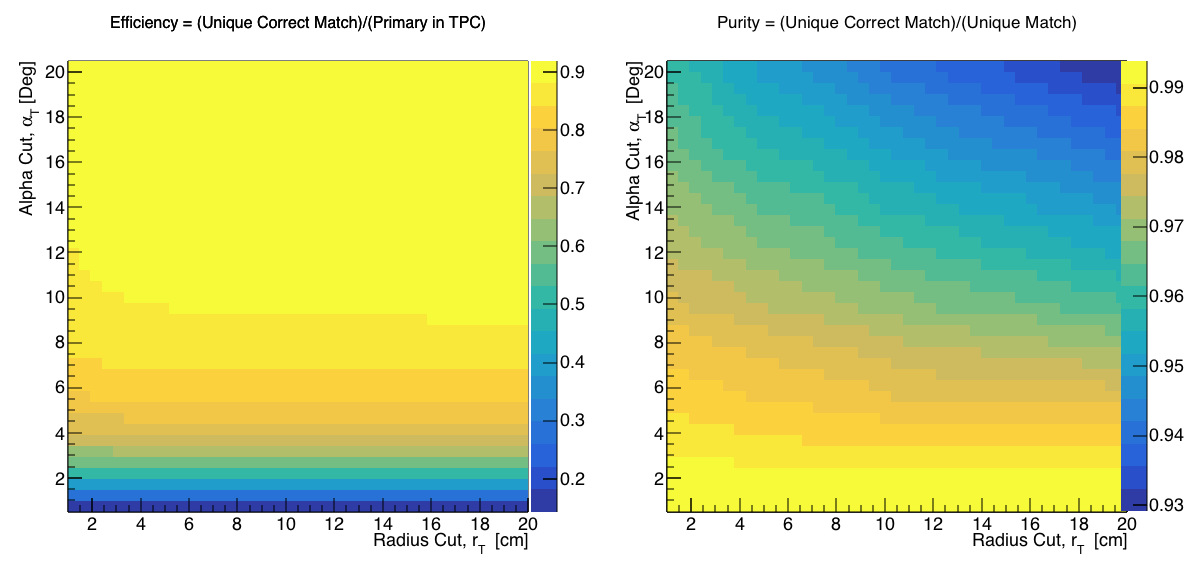
\includegraphics[width=15cm]{Chapter-5/Images/KEffPurity.png}
\caption{Efficiency (left) and purity (right) for wire chamber-to-TPC match as a function of the radius and angle selections.}
\label{fig:EffPurityK}
\end{figure}

\subsection{Interaction Point Optimization}\label{ch:TrackingOptimization}
Scheme of this subsection
\subsubsection{Brief Explanation of the reconstruction chain}
\subsubsection{Explanation of clustering parameters}
\subsubsection{Figure of merit and  spanning of cluster}
\subsubsection{Important numbers out of this optimization}


Plots I want in this section:
\begin{enumerate}
\item Delta L, reco - true
\item Delta L, reco - true Elastic, Delta L, reco - true Inelastic, other
\item Length Quality cut
\item Efficiency as a function of true KE and Angle
\end{enumerate}


\subsection{Tracking spatial and angular resolution}
Scope of this study is understanding and comparing the tracking spatial and angular resolution on data and MC.
We start by selecting all the WC2TPC matched tracks. 
We fit a line on all the space points of the track and calculate the $\chi^2$. The $\chi^2$ distribution for data and MC is shown in Figure \ref{fig:Chi2AllPts}.

For the spatial and angular resolution study, we reject tracks with less than 14 space points. For each track, we order the space points according to their Z position and we split them in two sets: the first set counts all the points belonging to the first half of the track and the second set counts all the points belonging to the second half of the track. We remove the last 5 points in the first set and the first 5 points in the second set, so to have a gap in the middle of the original track. We fit the first and the second set of points with a line separately. We reject the event entirely if the  $\chi^2$ for the fit of either of the halves is greater than four.  We define a track middle plane as the plane perpendicular to the original track fit, positioned in the middle of its length. We project the tracks on the middle plane and calculate the impact parameter, $d$, i.e. the distance between the projected points. We also calculate the angle between the original track direction and the fit of the first and second half, called $\alpha_1$ and $\alpha_2$ respectively. The spatial resolution of the track will be $\sigma_S = \frac{d}{\sqrt 2}$ while the angular resolution of the tracks will be  $\sigma_\alpha = \alpha_1 - \alpha_2$. The distributions for data and MC for $\sigma_\alpha$ and $\sigma_S$ are given in \ref{fig:trackingResolution}.




\end{comment}




